\chapter{Markovské řetězce}
\section{Absorpční Markovské řetězce}
Markovský řetězec je absorpční má-li alespoň jeden absorpční stav a je-li přechod z každého neabsorpčního stavu do absorpčního stavu možný. Neabsorpční stavy nazveme \textbf{tranzientními}. (Jakmile se jednou dostaneme do absorpčního stavu, zůstaneme tam již napořád).

\begin{figure}
\begin{tikzpicture}[->,>=stealth',thick, node distance = 4cm]
\node[state](a){$A$};
\node[state, right of = a](b) {$B$};
\node[state, below right of = a, node distance = 2cm](c){$C$};

\path (a) edge node[above]{$0.5$} (b)
	  (a) [bend left] edge node[above]{$0.5$}(c)
	  (c) [bend left] edge node[below]{$0.25$}(a);
\path[min distance = 1cm] (b) [loop above] edge node[above]{$1$}(b)
						  (a) [loop above] edge node[above]{$0.25$}(a)
						  (c) [loop right] edge node[right]{$0.5$}(c);
\end{tikzpicture}

\caption{Absorpční a tranzientní Markovské řetězce}
\end{figure}

Markovský řetězec skončí v absorpčním stavu s pravděpodobností 1. (Pokud bude absorpčních stavů více, nevíme, ve kterém skončíme, ale bude mít pravděpodobnost 1). Odpovídající matice je

\[ \vec{P} =
\begin{bmatrix}
\frac{1}{4} & \frac{1}{4} & \frac{1}{2}\\
\frac{1}{2} & \frac{1}{2} & 0\\
0 & 0 & 1
\end{bmatrix}
\]

\subsection{Základní úlohy}
\begin{enumerate}[label=\arabic*)]
\item \textbf{pravděpodobnost, že Markovský řetězec skončí v daném absorpčním stavu}\br

	Nechť má Markovský řetězec $s$ stavů, z toho $r$ absorpčních a tímpádem $s-r$ je tranzientních. Máme k dispozici matici přechodu $\vec{P}$ je velikosti $s\times s$. Předpokládáme, že Markovský řetězec startuje z tranzientního stavu $a_i$ a ptáme se, s jakou pravděpodobností skončí v určitém absorpčním stavu $a$. Tuto pravděpodobnost označíme $d_i$. Pravděpodobnost, že Markovský řetězec přejde v jednom kroku ze stavu $a_i$ do stavu $a_j$ a potom přejde do stavu $a$, spočteme jako $P_{ij}\cdot d_j$ (ppst že MŘ přejde z $a_i$ do $a_j$ a potom do $a$). Úplná pravděpodobnost přechodu z $a_i$ do $a$ je

	\[ d_i=p_{i1}\cdot d_1+ p_{i2}\cdot d_2 + \ldots + p_{ij}\cdot d_s \]

	Maticový přepis této rovnice nám říká, že

	\[ \vec{d} = \vec{P}\vec{d},\quad \vec{d}=[d_1,d_2,\ldots,d_s] \]

	Tato soustava má více řešení. Vybíráme z nich jediný vektor $d$ tak, aby jeho prvek, odpovídající danému absorpčnímu stavu,  byl jedna a prvky odpovídající ostatním absorpčním stavům byly nulové. Pokud máme víc absorčních stavů, získaneme více vektorů $d$.

	\begin{note}{Příklad}
		Vektor $\vec{d}\t=[d_1,d_2,d_3,d_4,d_5]$, kde $d_1,d_5$ jsou absorpční stavy, $d_2,d_3,d_4$ jsou tranzientní stavy. Pravděpodobnost, že se dostanu do $d_1$ je
		\[ \vec{P} = [1,\cdot,\cdot,\cdot,0] \]

	\end{note}

\item \textbf{střední počet přechodů přes daný tranzientní stav}\br

	Nechť $t_{ij}$ označuje středí počet přechodů při startu z tranzientního stavu $a_i$ přes stav $a_j$ než se dostaneme do absorčního stavu.

	\[ t_{ij}=p_{i1}t_{1j}+p_{i2}t_{2j}+\ldots+p_{i,s-r}t_{s-r,j}+\delta_{ij} \]

	\[ \delta_{ij}=
	\begin{cases}
	1 & i=j\\
	0 & i\neq j; i,j = 1,\ldots, s-r
	\end{cases}
	\]

	(Důvod $\delta_{ij}$ je, že se výchozí stav započítává do počtu přechodů, pokud tam náhodou začínáme). Maticový zápis

	\[ \vec{T} = \vec{Q}\cdot\vec{T}+\vec{I} \]

	Matice přechodu $\vec{Q}$ vznikne z $\vec{P}$ vynecháním řádků a sloupců odpovídajícím absorpčním stavům, tj. $\vec{Q}$ je matice velikosti $(s-r) \times (s-r))$. Řešení je tedy

	\[ \vec{I}=(\vec{I}-\vec{Q})\cdot\vec{T}\Rightarrow \vec{T}=(\vec{I}-\vec{Q})^{-1} \]

\item \textbf{střední počet přechodů přes všechny tranzientní stavy před skončením ve stavu absorpčním}\br

	Využijeme znalosti z předchozí úlohy. $t_{ij}$ udává střední dobu (pokud se přechody uskutečňují ve stejných časových okamžicích) strávenou ve stavu $a_j$, pokud startujeme ze stavu $a_i$.

	\[ t_i=\sum_{j=1}^{s-r}t_{2j} \]

	Doba (střední počet průchodů) pobytu v tranzientních stavech před pohlcením v absorpčním stavu je

	\[ t = \vec{T}\cdot
	\begin{bmatrix}
	1\\1\\1\\1
	\end{bmatrix}
	\]
\end{enumerate}

\section{Bernoulliho řada}
Bernoulliho řada je množina nezávislých náhodných proměnných se stejným rozložením $[X(0),X(1),\ldots]$ a s hodnotami $\brs{0,1}$, kde $P(X(k)=1)=p$ a $P(X(k)=0)=q=1-p$. Tato řada je \textbf{stacionární} a platí

\[ \mean{X(k)}=p,\mean{X^2(k)}=p, \]
\[ \var{X(k)}=p-p^2=p(1-p)=p\cdot q  \]

Stejné pro Bernoulliho Náhodnou Veličinu, protože hustota pravděpodobnosti je stejná pro všechny časové okamžiky.

Pokud budou hodnoty $\brs{-1,1}$, jedná se o symetrickou Bernoulliho proces/řadu. Velice jednoduchý typ náhodného procesu, jedná se o přiřazení indexu náhodným proměnným, které jsou nezávislé a mají stejná rozložení. Složitější náhodné procesy lze generovat tak, že na vstup nějakého systému (filtr) aplikujeme tyto jednoduché procesy a na výstupu získáme korelované procesy.

\begin{figure}
\begin{tikzpicture}[->,>=stealth',thick,node distance = 2cm]
\node[input](in){};
\node[block, right of = in](filtr){filtr};
\node[output, right of = filtr](out){};

\path (in) edge node[below left]{nekorelovaný proces}(filtr)
	  (filtr) edge node[below right]{korelovaný proces}(out);
\end{tikzpicture}
\caption{Generování korelovaných procesů}
\end{figure}

\section{Bernoulliho náhodná procházka}
Nechť $W(k)$ je symetrický Bernoulliho process s hodnotami $\brs{-1,1}$ takový, že

\[ P(W(k)=1) = p = P(W(k)=-1)=q=\frac{1}{2} \]

Náhodná řada

\[ X(k) = \sum_{m=1}^k W(m) \]

a $X(0)=0$ a $W(0)=0$ je \textbf{Bernoulliho náhodná procházka}.

\begin{figure}
	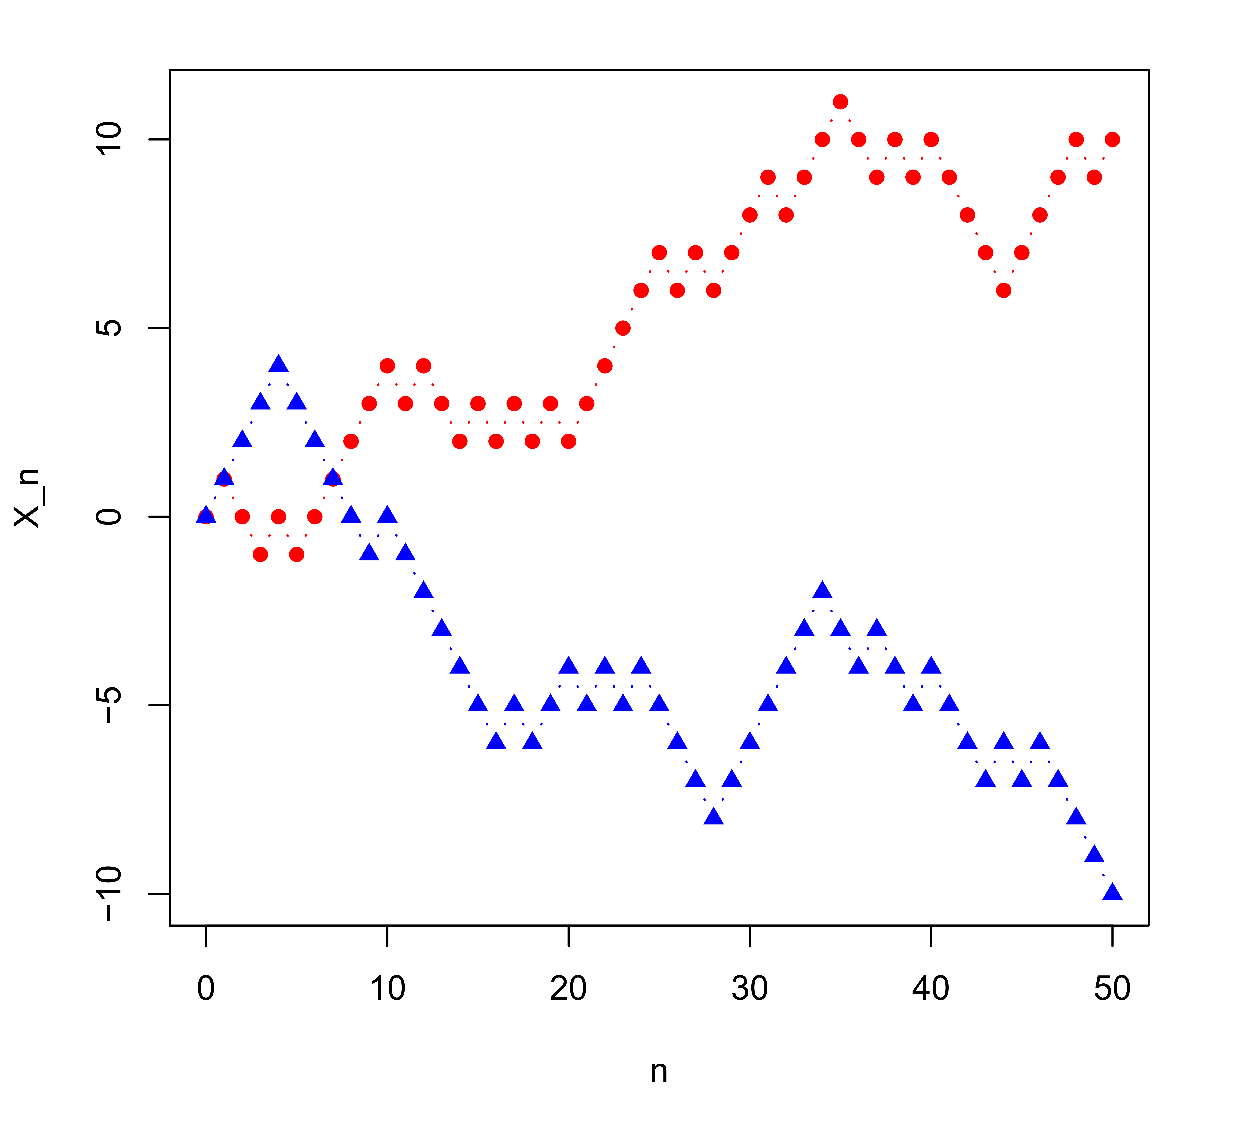
\includegraphics[scale=0.3]{obrazky/random_walk.png}
	\caption{Akumulovaný majetek hráče po $k$-té hře, fenomén teplotního šumu}
\end{figure}

Součet nemá Bernoulliho rozložení a nabývá hodnot v oboru celých čísel \textbf{Z}). Definiční vztah lze přepsat

\[ X(k) =X(k-1)+W(k), \]

což je filtr s nekonečnou impulsní odezvou, s pólem $z=1$. Momenty Bernoulliovy řady $\mean{W(k)}=0,\mean{W^2(k)}=1$, momenty náhodné procházky

\begin{eqnarray*}
\mean{X(k)} & = & \mean{\sum W(m)} =  \sum \mean{W(m)} = \sum 0 = 0\\
\mean{X^2(k)} & = & \mean{\left(\sum_{m=1}^k W(m)\right)\cdot\left(\sum_{n=1}^k W(n)\right)}=\\
& = & \mean{\sum_m^k\sum_n^k W(m)W(n)}=\\
& = & \sum^{k,k}_{\substack{m,n\\m\neq n}}\underbrace{\mean{W(m)}}_0 \underbrace{\mean{W(n)}}_0+K = K
\end{eqnarray*}

Platí $\var{X(k)}= \mean{X^2(k)} - \mean{X(k)}^2 = \mean{X^2(k)} - 0^2 =  K$. Variance roste lineárně, proces není stacionární. Autokorelační funkce je ve tvaru

\begin{eqnarray*}
R_{xx}(k_1,k_2) &=& \mean{X(k_1)\cdot X(k_2)}=\mean{\left(\sum_{m=1}^{k_1}W(m)\right)\left(\sum_{n=1}^{k_2}W(n)\right)}=\text{momenty}=\\
& = & \min(k_1,k_2)
\end{eqnarray*}

Pokud to $W(k)$ je Bernoulliho řada bez symetrických hodnot s $ \brs{0,1} $ pak neříkáme Bernoulliho procházka, ale binomická sčítací řada.



\subsection{Poissonův sčítací proces}

Proces spojitý v čase, diskrétní

definujme časový interval $ \Delta t = \frac{t}{k} \;\;\;\; k \in T = R^k, k \in N$

a uvažujme náhodný proces $X(t) \in X(k \Delta t)$, kde $X(k \cdot 1)$ je bermouliho sčítací řada.

Taková definice procesu umožnuje zobecnění, kdy úspěch může nastav v libovolně dlouhém intervalu, ne pouze pro $ \Delta t = 1$

Uvažujme následující podmínky:
\begin{itemize}
	\item $X(k \Delta t)$ je binomická náhodná veličina s pavděpodobností úspěchu $p$ uměrnou délce intervalu $$ p =P (X(\Delta t) = 1) = \lambda \Delta t$$ kde $\lambda$ je parametr rychlosti.
	\item interval $\Delta t$ je dostatečně malý, aby v libovolném intervalu nastal úspěch pouze jednou. Pravděpodobnost výskytu úspěchu v jednom intervalu je roven $0$.
\end{itemize}

Potom $X(t)$ je Poissonův sčítací proces.


Jaká je ppst že v čase $t$ máme hodnotu $n$

\[ P(X(k \Delta t) = n) = (\lambda \Delta t)^n \cdot (1 - \lambda\Delta t)^{k-n} \]

Nechť $k \rightarrow \infty$, potom $\Delta t \rightarrow 0$ a tedy pravděpodobnost $P = \lambda \Delta t = 0$
ale střední hodnota musí být konečná.

\[ P \cdot k = \lambda \Delta t k = \lambda \frac{t}{k} k = \lambda t \]

aproximace

\[ P(X(t)=n) \approx \dfrac{(\lambda t)^n}{n!} e^{-\lambda t} \;\;\; n \in Z^+ \]

což je Poissonovo rozdělení s časově proměným parametrem $ \Delta t$

Definice Poissonův sčítací proces $X(t)$ je Náhodná Veličina diskrétní v úrovni, spojitý v čase s $X(0)=0$ takový, že ppst úspěchu v čase $t$ je dán Poissonovým rozdělením s parametrem $ \alpha = \lambda t$

pozn. na rozdíl od binomické sčítací čady může změna nastat v libovolném časovém okamžiku.

% \begin{figure}
% 	\includegraphics[scale=0.3]{obrazky/poisson_walk.png}
% \caption{Průběh poissonovi procházky}
% \end{figure}

Momenty:

\begin{itemize}
	\item $\mean{X(t)} = \lambda t$
	\item $\var{X(t)} = \lambda t$
\end{itemize}
Jde tedy o nestacionární proces

Příklady
\begin{itemize}
	\item přesný model radioaktivního rozpadu
	\item počet poruch na telefoní lince
	\item příchod zákazníků do obchodu
	\item Př. emaily jsou doručovány podle Poissonova procesu s rychlostí $\lambda = 0.2$ zpráv za hodinu. A emaily kontrolujete jednou za hodinu, jaká je ppst že nenajdete novou zprávu v inboxu? \[ P(1) = 0) = \dfrac{(-0.2 \cdot 1 )^0}{0!} e^{-0.2 \cdot 1} = 0.819 \] další \[ P(1) = 0) = \dfrac{(-0.2 \cdot 1 )^1}{1!} e^{-0.2 \cdot 1} = 0.164 \]
\end{itemize}

Zaměřme se na dobu mezi dvěma událostmi.

Poissonův proces je ISI (Indenpendent stacionary increments), můžeme tedy zkoumat libovolný časový interval

např. čas první události (označíme jí $\vec{Y}$ je to Náhodná veličina), pokud je čas první události větší než $t$, pak na intervalu $<0,t>$ je 0 událostí \[ P(Y>t) = P(X(t) = 0) = e^{-\lambda t} \;\;\;\; t >= 0 \]
pak \[ F_Y(t) = P(Y <= t ) = 1 - e^{-\lambda t} \]

což je  distribuční funkce s exponenciálním rozdělení \[ \mean{\vec{Y}} = \frac{1}{\lambda}, \;\;\; \var{\vec{Y}} = \frac{1}{\lambda^2} \]
jaká bude distribuční funkce času, než nastane $n$-tá událost (ozn. $\vec{Y_n}$)

Protože jsou intervali mezi událostmi nezávyslé, lze $\vec{Y_n}$ vyjádřit  součtem intervalů \[ \vec{Y_n} = \sum_{k=1}^n (\vec{Y_k} -\vec{Y_{k-1}}) \]

$\vec{Y_n}$ je tedy součet nezávislých náhodných veličin s exponenciálním rozdělením a má Erlangovo rozdělení \[ P_{\vec{Y_k}} (t) = \dfrac{\lambda^n t^{k-1}}{(n-1)!} e^{-\lambda t} \;\;\;\; t >= 0 \]

Momenty: \[ \mean{Y_n} = \frac{n}{\lambda},  \;\;\;\; \var{Y_n} = \frac{n}{\lambda}  \]

%V simulinku realizovat dirachovy pulsi s intervalem byl exponencialně rozložen, na výstupu integrátoru bude


\subsubsection{Autokovarianční (autokorelační) fce Poiss. processu}
\label{subs:Autokovarianční (autokorelační) fce Poiss. processu}

potřebujeme sdruženou hustotu ppsti pro dva časové okamžiky ($t_1$ a $t_2$), nečhť $t_2 > t_1$

\[ P(X(t_1) = n_1, X(t_2) = n_2) = P(X(t_2)=n_2 | X(t_1)=n_1 ) P(X(t_2)=n_1 ) \]


díky bezpamětovostí exponenciálního rozdělení

\[ P(X ) n+ x | X > n) P(X>x) \]

má podmíněná pravděpodobnost $P(X(t_2)=n_2| X(t_1)=n_1)$ Erlangovo rozdělení s parametry $\lambda (t_2 -t_1)$ a $r = n_2 - n_1$

Pokud by do okamžiku by do $t_1$ nastalo $n_1$ událostí, pak rozložení závisí na zbylém počtu $n_2-n_1$ v průběhu časového okamžiku $<t_1,t_2>$



\begin{align}
	P(X(t_1) = n_1, P(X(t_2)=n_2) &= \dfrac{\lambda (t_2-t_1)}{(n_2-n_1)} \cdot e^{-\lambda (t_2-t_1)} \cdot e^{-\lambda t_1} \\ &= \dfrac{1}{n_2} [\lambda(t_2-t_1)]^{n_2-n_1} (\lambda t_1)^{n_1}  {n_2 \choose n_1} e^{-\lambda t_2}
\end{align}


\section{Wienerův proces}
Wienerův proces je model fyzikálního jevu známého jako Braunův pohyb, kde se částice chaoticky pohybuje v kapalině díky náhodným srážkám s molekulami kapaliny. Wienerův proces lze odvodit z Bernoulliho řady, která nabývá hodnot $\brs{-\varepsilon,\varepsilon}$ pro malé $\varepsilon>0$. Předpokládejme, že se kolize odehrávají s rychlostí $\alpha$, tzn. odehrávají se v násobcích $\frac{1}{\alpha}$. Celkový počet kolizí za čas $t$ je $n=\lfloor\alpha\cdot t\rfloor$ (zaokrouhlování dolů na celá čísla).

\subsubsection*{Definujeme náhodný proces}
\[ X(t)=\sum_{m=1}^{\lfloor\alpha\cdot t\rfloor} W(m), \]

který je podobný Bernoulliho náhodné procházce, ale

\begin{enumerate}[label=\roman*)]
\item intervaly mezi událostmi jsou $\frac{1}{\alpha}$ namísto 1.
\item amplitudy jsou $\brs{-\varepsilon,\varepsilon}$ namísto $\brs{-1,1}$
\item horní mez je $\lfloor\alpha\cdot t\rfloor$ namísto $k$
\end{enumerate}

Wienerův proces se získá limitním přechodem $\varphi\to 0$ (spojitý náhodný proces) a $\frac{1}{\alpha}\to 0$ (proces spojitý v čase).

\[ Y(t) = \lim_{\substack{\varepsilon\to 0\\ \frac{1}{\alpha}\to 0}} X(t) \]

Jak budou vypadat momenty po limitním přechodu:

\[ \mean{Y(t)} = \lim_{\substack{\varepsilon\to 0\\ \frac{1}{\alpha}\to 0}} \mean{X(t)}=0 \]

Z toho plyne, že Wienerův proces má trvale nulovou střední hodnotu. V případě variace

\[ \mean{Y^2(t)} = \lim_{\substack{\varepsilon\to 0\\ \frac{1}{\alpha}\to 0}} \mean{X^2(t)}=\lim_{\substack{\varepsilon\to 0\\ \frac{1}{\alpha}\to 0}} \lfloor\alpha t\rfloor \varepsilon^2 \]

pro $\frac{1}{\alpha}\to 0, \lfloor\alpha t\rfloor=\alpha t$. Vztah upravíme vytknutím $t$ a tedy

\[ \mean{Y^2(t)} = t \lim_{\substack{\varepsilon\to 0\\ \frac{1}{\alpha}\to 0}} \frac{\varepsilon^2}{\frac{1}{\alpha}} \]

Aby měl proces smysl, musí $\mean{Y^2(t)}>0$ a zároveň $\mean{Y^2(t)}<\infty$. Proto musí $\frac{1}{\alpha}\to 0$ a $\varepsilon^2\to 0$ řádově stejně rychle.

\subsection{Definice Wienerova procesu}
Wienerův proces je náhodný proces spojitý v čase popsaný gaussovskou hustotou pravděpodobnosti (normální rozdělení), nebo:

\[ P_{x(t)}(x)=\frac{1}{\sqrt{2\pi\alpha\varepsilon^2 t}}e^{-\frac{x^2}{2\alpha\varepsilon^2 t}}, \]

která má nulovou střední hodnotu a varianci $\sigma^2_\lambda(t) = \alpha\varepsilon^2 t$. Počáteční podmínka Wienerova procesu je $P(X(t)=0)=1$ \uv{začínáme z nuly}. Je to proces spojitý v čase a v úrovni. Odpovídá výstupu integrátoru. Korelační a autokovarianční funkce jsou stejné z důvodu 0 středních hodnot, tedy

\begin{eqnarray*}
R_{xx}(t_1,t_2) &=&\mean{X(t_1)X(t_2)} = \mean{X(t_1)\cdot[X(t_1)+X(t_2)-X(t_1)]} = \\
& = & \mean{X^2(t_1)} + \mean{X(t_1)\cdot(\underbrace{X(t_2)-X(t_1)}_{\text{nezávislý přírůstek}})}= \\
& = & \mean{X^2(t)}+\underbrace{\mean{X(t_1)}}_0\cdot \underbrace{\mean{X(t_2)-X(t_1)}}_0 = \alpha\varepsilon t_1
\end{eqnarray*}

Předpokladem je $t_1<t_2$

Wienerův proces má stacionární nezávislé přírustky!

Často se označuje $\alpha\varepsilon^2 \triangleq \sigma^2$